\scanpage{13}\mspage{12}
\deleted{\unsure{pre|pr}}inclure soit $\leq$, soit $\triangleleft$.

\deleted{b) $\leq$ et $\ll$ \unsure{déterminent} $\preccurlyeq$, car}
\[
\deleted{G\preccurlyeq F\Longleftrightarrow G\ll F}
\]

b) Chacune des relations $\leq$, $\ll$ détermine la relation $\parallel$. En effet
\[
\left\{\begin{aligned}
\text{a)}\quad F\parallel G &\ \deleted{\unsure{\Longleftrightarrow|\Longrightarrow}}\unsure{\Longrightarrow|\Longleftrightarrow}
 \{F,G\}\ \text{majoré pour }\leq,\ \text{et }\mathop{\mathrm{Inf}}\limits_{\leq}(F,G)=\varnothing_F\\
\text{b)}\quad F\parallel G &\ \Longleftrightarrow
 \deleted{\unsure{\mathrm{Inf}|\mathrm{S}}}\mathop{\mathrm{Sup}}\limits_{\ll}(F,G)\ \text{existe, et }\mathop{\mathrm{Inf}}\limits_{\ll} F,G=\varnothing_F
\end{aligned}\right.
\tag*{(1.24)}
\]
\margin{Verifier $\longrightarrow$}
(\uline{NB} $\varnothing_{\unsure{\mathcal{F}|\mathfrak{F}}}$ est à la fois plus petit \unsure{elémt|elément} de $\mathcal{F}$ pour $\leq$, et pour $\ll$)

c) La relation $\ll$ détermine $\preccurlyeq$, par
\margin{$\times$}
\[
\begin{aligned}
F\preccurlyeq G &\Longleftrightarrow F\ll G,\ \text{et }\forall H\underset{\deleted{\leq}}{\in}\mathcal{F}\deleted{\unsure{H|K}}\ \text{on a}\\
&\hspace{2em}(H\parallel F\Longleftrightarrow H\parallel G)
\end{aligned}
\tag*{(1.25)}
\]
et on applique b).

d) La relation $\ll$ détermine $\mathcal{L}\subset\mathcal{F}$ comme l'\unsure{ens} des éléments minimaux de $\mathcal{F}\setminus\{\varnothing_{\mathcal{F}}\}$ :
\[
\mathcal{L}=\bigl\{\substack{X\in\mathcal{F}\\ X\neq\varnothing_{\mathcal{F}}}\mid
 Y\in\mathcal{F},\ Y\ll X,\ Y\neq\varnothing_{\unsure{\mathcal{F}|F|f}}\ \Rightarrow Y=X\bigr\} \tag*{(1.26)}
\]
(un \unsure{lieu|lien} est une figure non vide dont le seul raffinement non vide est elle-$\overline{\mathrm m}$).

\figure{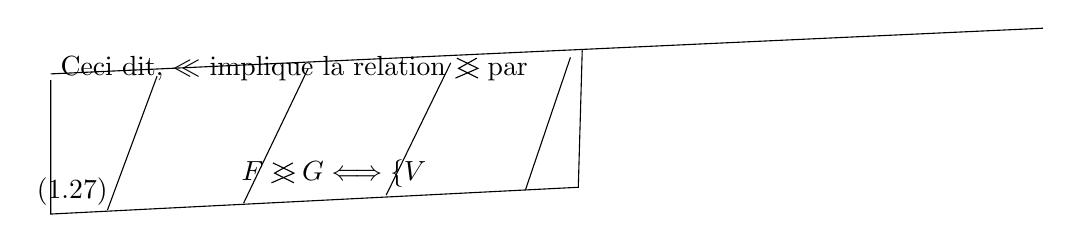
\begin{tikzpicture}[x=1cm,y=1cm]
\node[anchor=west] at (0,1.55) {\deleted{Ceci dit, $\ll$ implique la relation $\mathrel{\tikz[baseline=0pt,x=1em,y=1em]{\draw (-.38,.62)--(.38,.25)--(-.43,-.10); \draw (.34,.62)--(-.32,.25)--(.38,-.10);}}$ par}};
\node[anchor=west] at (-.3,-.02) {$\deleted{(1.27)}$};
\node[anchor=west] at (2.3,.22) {$\deleted{F \mathrel{\tikz[baseline=0pt,x=1em,y=1em]{\draw (-.38,.62)--(.38,.25)--(-.43,-.10); \draw (.34,.62)--(-.32,.25)--(.38,-.10);}} G\Longleftrightarrow\{V}$};
\draw (0,1.48)--(12.6,2.06);
\draw (0,1.40)--(0,-.30)--(6.7,.04)--(6.75,1.78);
\draw (.72,-.25)--(1.35,1.45);
\draw (2.45,-.16)--(3.27,1.55);
\draw (4.26,-.06)--(5.08,1.62);
\draw (6.03,.01)--(6.60,1.69);
\end{tikzpicture}}
Je ne vois pas que $\ll$ ($+\ \preccurlyeq$, c'est kif-kif) détermine $\leq$, ni même $\mathrel{\tikz[baseline=0pt,x=1em,y=1em]{\draw (-.38,.62)--(.38,.25)--(-.43,-.10); \draw (.34,.62)--(-.32,.25)--(.38,-.10);}}$. Mais

\textcircled{\unsure{e|$\ominus$}}\quad $\ll$ et $\mathrel{\tikz[baseline=0pt,x=1em,y=1em]{\draw (-.38,.62)--(.38,.25)--(-.43,-.10); \draw (.34,.62)--(-.32,.25)--(.38,-.10);}}$ déterminent $\leq$ par
\margin{$\times$}
\[
G\leq F\quad\unsure{\Longleftarrow|\Longleftrightarrow}\quad (G\ll F\ \text{et}\ G \mathrel{\tikz[baseline=0pt,x=1em,y=1em]{\draw (-.38,.62)--(.38,.25)--(-.43,-.10); \draw (.34,.62)--(-.32,.25)--(.38,-.10);}} F) \tag*{(1.27)}
\]

Donc finalement,
